\overlays{2}{

\begin{slide}{L'interfaccia grafica}
{\small
GNU/Linux ha una potentissima modalità grafica che si basa su un
componente chiave: \emph{Xorg}.

\onlySlide*{1}{
La più importante caratteristica di Xorg è che è \emph{network-based}.
Che vuol dire? Vuol dire che tutte le operazioni vengono svolte via
rete.

Xorg si compone di un server e di tanti client.
}

\onlySlide*{2}{
	\flushright{ 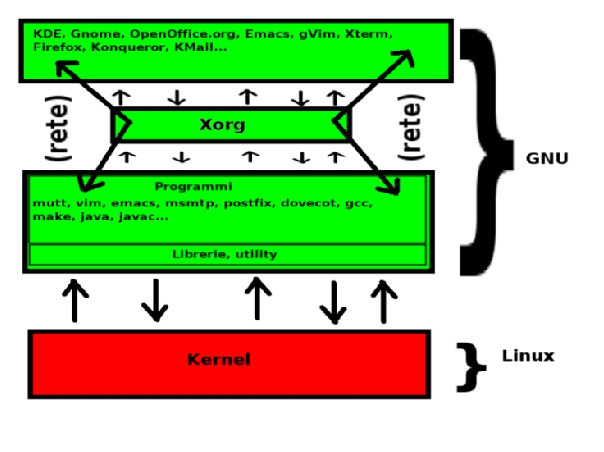
\includegraphics[width=8cm,height=6cm]{immagini/xorg_layout.eps} }
}

}

\end{slide}}
